\section{KA Prior (Modality--Agnostic)}
\label{app:ka-contract-theory}

In this part we describe regime conditions and operator-level sufficient structure for a knowledge-aided (KA) temporal covariance transform layered on top of a baseline slow-time detector. The analysis is formulated in terms of abstract band projectors $(\Po,\Pf,\Pg,\Pa)$, alias features, and score distributions, and does not depend on any particular imaging modality. Only in later sections do we instantiate these conditions for functional ultrasound (fUS) brain imaging with concrete band choices, acquisition parameters, and baselines.

\subsection*{How to read this appendix (plain-English map)}
This appendix lists explicit preconditions under which the KA prior is allowed to modify scores; if any precondition fails, the prior is disabled ($w\equiv 1$; KA off). The labels below are grouped by purpose.

\begin{table}[t]
\centering
\small
\begin{tabular}{p{2.2cm} p{12.4cm}}
\hline
Label group & Plain-English meaning (what it checks) \\
\hline
R--* & Regime preconditions: do the bands exist, do risk features vary, and is there tail headroom worth regularizing? \\
BG--* & Band geometry: after discretization, are Pf/guard/Pa non-empty and non-overlapping for the chosen (PRF, $T$)? \\
OC--* & Operator/covariance constraints: KA can only apply bounded, bandwise structure without uncontrolled mixing or conditioning pathologies. \\
G--* & Gating/localization: KA is allowed to act only where artifacts are likely and positives are unlikely (protected/do-not-penalize set preserved; scores unchanged). \\
Safety--* & Safety guards: if any check indicates score inflation or loss of invariance, KA is forced off. \\
\hline
\end{tabular}
\caption{Appendix label groups in plain English. Failing any condition triggers a conservative fallback ($w=1$), which is an intended success mode out of regime.}
\end{table}

\begin{figure}[t]
\centering
\IfFileExists{figs/paper/stap_pipeline_bayes_block.pdf}{%
  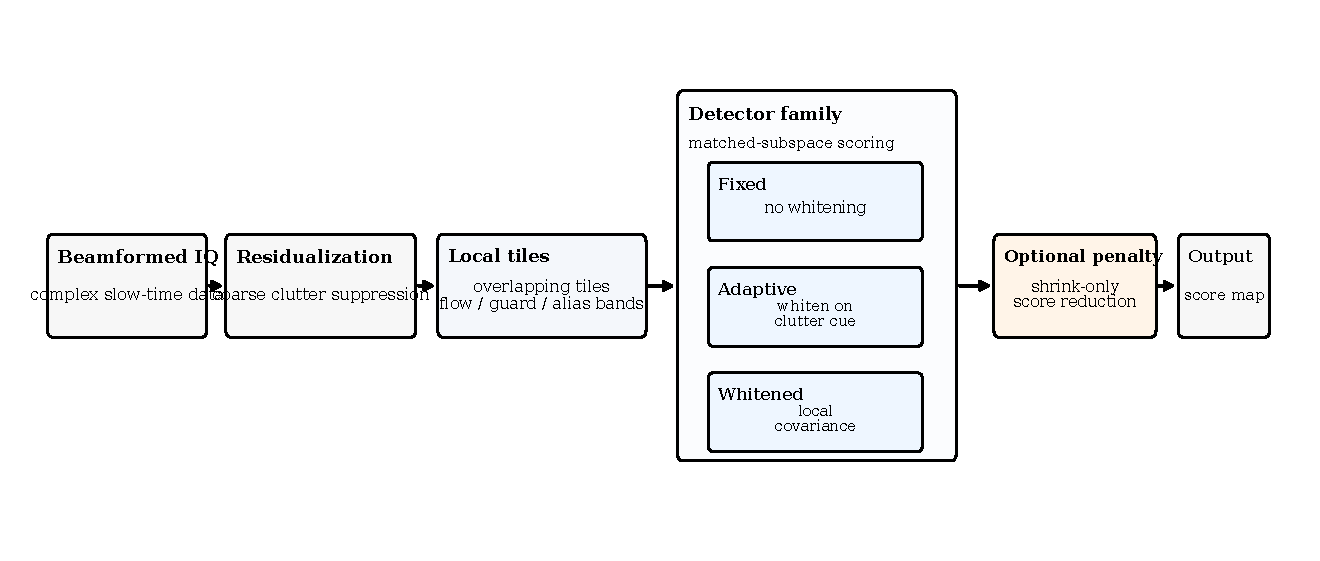
\includegraphics[width=\linewidth]{figs/paper/stap_pipeline_bayes_block.pdf}%
}{%
  \fbox{\begin{minipage}{0.95\linewidth}
    \centering
    \vspace{0.5em}
    Missing figure \path{figs/paper/stap_pipeline_bayes_block.pdf}.\\
    Reproduce it with \path{PYTHONPATH=. python scripts/fig_stap_pipeline_bayes_block.py}.
    \vspace{0.5em}
  \end{minipage}}%
}
\caption{System block diagram for the Knowledge-Aided Space-Time Adaptive Processing (KA--STAP) architecture. Beamformed kilohertz data initially undergoes baseline motion-compensated clutter filtering (MC--SVD), yielding a residual cube $X_{\mathrm{base}}$. The residual is processed via two parallel branches: (top) the uninformed STAP core computes the matched-subspace statistic $S_{\mathrm{stap,pre}}(y,x)$; (bottom) a spatial-spectral feature extractor evaluates localized band-energy statistics to compute a bounded shrink-only weight $w(i)\in(0,1]$ (equivalently $\gamma(i)=1/w(i)\geq 1$). The branches recombine to form the strictly bounded post-regularization score $S_{\mathrm{stap,post}}(y,x)=w\,S_{\mathrm{stap,pre}}(y,x)$ (shrink-only).}
\label{fig:stap_pipeline}
\end{figure}

\subsection{Regime Preconditions (Data--Level, Non--Negotiable)}
\label{sec:regime}

The most important empirical lesson is: even if the KA operator $Q$ and band design $(\Pf,\Pa)$ are perfect in an abstract sense, \emph{uplift requires the data themselves to be in a compatible regime}. This section codifies that.

We write $S(f)$ for the (multi--taper) PSD of a baseline--whitened tile, and define
\[
E_f := \sum_{f\in\Cf} S(f),\quad
E_a := \sum_{f\in\Ca} S(f),\quad
E_g := \sum_{f\in\Cg} S(f),
\]
with $\Cf,\Ca,\Cg$ the flow, alias, and guard bands in frequency.

\subsection{R--1: Band Occupancy Separation}

We require that the fixed bands $(\Cf,\Ca)$ are physically meaningful for the current PRF, slow--time length $T$, and DPSS parameters, in the sense that label statistics show actual occupancy.

On a held--out labeled sample:
\begin{align}
\mathbb{P}\!\left\{f_{\mathrm{peak}}\in\Cf \;\middle|\; H_1\right\} &\ge p_{f,\min},\qquad p_{f,\min}\in [0.5,0.7],\\[0.5ex]
\mathbb{P}\!\left\{f_{\mathrm{peak}}\in\Ca \;\middle|\; H_0\right\} &\ge p_{a,\min},\qquad p_{a,\min}\in [0.2,0.3],
\end{align}
where $f_{\mathrm{peak}}$ is the frequency at which $S(f)$ attains its maximum and $H_1$/$H_0$ denote flow/background tiles.

Interpretation: a majority of flow tiles have their dominant PSD peak \emph{inside} the flow band, and a nontrivial fraction of background tiles have their dominant peak in the alias band. This ensures that the band projectors $(\Pf,\Pa)$ actually correspond to distinct physical processes.

\paragraph{Implementation in labeled brain simulation profiles.}
For the main labeled brain simulation regimes, the raw k-Wave RF tensor $x(t,a,e)$ (angle index $a$, element index $e$) lives on an angle and element grid that does not align pixelwise with the STAP PD masks $(N_y\times N_x)$. We therefore implement R--1 using the whitened multi--taper PSD and band-ratio feature statistics computed on the \emph{same} spatial grid as the exported PD scoring maps (the right-tail score $S_{\mathrm{PD}}$ stored as \texttt{score\_pd\_*.npy}). We take $f_{\mathrm{peak}}$ from the whitened PSD peaks used in the band-ratio recorder and report the fraction of $H_1$ tiles whose peak lies in $\Cf$ and the fraction of $H_0$ tiles whose peak lies in $\Ca$ from those tilewise peak statistics. When the RF tensor is spatially aligned with the masks (e.g.\ 1D pilots), we instead use a direct FFT on $x(t,\cdot,\cdot)$ as in the definition above.

\subsection{R--2: Alias Score Class Separation}

We generalize the alias metric used for localization.

\paragraph{Alias score.} Let $m_{\text{alias}}(z)$ be any scalar score derived from the baseline PSD and/or covariance satisfying:
\begin{itemize}[nosep]
  \item $m_{\text{alias}}$ increases when $E_a$ grows relative to $E_f$,
  \item $m_{\text{alias}}$ is larger when Pa energy is more coherent or concentrated (e.g.\ a strong tone),
  \item $m_{\text{alias}}$ is penalized when guard/edge energy $E_g$ is large.
\end{itemize}
Examples (not exhaustive):
\begin{itemize}[nosep]
  \item Log band ratio: $m_{\text{alias}}(z) = \log\frac{E_a+\epsilon}{E_f+\epsilon}$,
  \item Combination of band fractions: $m_{\text{alias}}(z) = \frac{E_a}{E_f+E_a+E_g} \cdot c_a$ where $c_a$ is an alias--band coherence metric (e.g.\ leading eigenvalue fraction of a band--restricted covariance),
  \item Peak--location based scores (peak in Pa, high tone prominence).
\end{itemize}

For KA to be meaningfully guided by alias evidence, we require \emph{class--differential separation} of $m_{\text{alias}}$:
\begin{equation}
\label{eq:R2}
\operatorname{median}\!\left(m_{\text{alias}}\mid H_0\right) - \operatorname{median}\!\left(m_{\text{alias}}\mid H_1\right) \;\ge\; \Delta_{\min},
\end{equation}
with $\Delta_{\min}$ set so that alias dominance differs by at least a factor $\approx e^{\Delta_{\min}}$ in expectation (for log ratio, $\Delta_{\min}\approx 0.3$ corresponds to a $\approx 35\%$ relative difference in $E_a/E_f$ medians).

If \eqref{eq:R2} fails (alias score almost identical on $H_0$ and $H_1$), the alias-localization rule (Appendix~\ref{app:gating}) has no reliable signal and KA uplift cannot be expected.

\subsection{R--3: Baseline Headroom}

Let $S^-$ be the baseline score distribution on negatives, and $\text{pAUC}_\text{base}(\alpha)$ be the partial AUC up to FPR $\alpha$.

We require:
\begin{itemize}[nosep]
  \item Sufficient \emph{quantile density} at the target FPR $\alpha$ (as already assumed implicitly in SL--2): the density $f_-(t_\alpha)$ at the $\alpha$--quantile $t_\alpha$ is bounded away from 0.
  \item Baseline not already numerically saturated: for a chosen $\alpha_{\max}$ (e.g.\ $10^{-3}$),
  \[
    \text{pAUC}_\text{base}(\alpha\le \alpha_{\max}) \le \text{pAUC}_{\max} - \varepsilon_{\text{AUC}},\qquad \varepsilon_{\text{AUC}}>0,
  \]
  where $\text{pAUC}_{\max}$ is the ideal partial AUC under perfect separation.
\end{itemize}

If the baseline already achieves near--maximal pAUC at the FPR of interest, even a perfect KA transform cannot provide significant gains; in this regime KA can serve as a regularizer or safety mechanism, but not as a source of measurable uplift.

\subsection{Operator--Level Sufficient Structure (Non--Negotiable Core)}
\label{sec:operator}

This section is unchanged at the core: it describes conditions on $Q$ alone under which KA behaves like a band--wise scalar rescaling of scores, up to small perturbations.

\subsection{OC--1: Approximate Band Commutation}

We require $Q$ to be nearly block--diagonal with respect to $(\Po,\Pf,\Pg,\Pa)$:
\[
\Norm{[Q,\Pf]}_2 \le \varepsilon_{\text{mix}},\qquad
\Norm{[Q,\Pa]}_2 \le \varepsilon_{\text{mix}},
\]
for some small $\varepsilon_{\text{mix}}\in[0,1)$ (typical target $\le 0.05$).

Interpretation: $Q$ preserves band subspaces up to small mixing; it does not rotate energy from Pf into Pa or vice versa in any substantial way. This rules out the failure mode where KA accidentally feeds alias into the flow numerator.

\paragraph{Runtime label--free check.}
Let $\wh Q := R_\beta^{-1/2}\wh R^{1/2}$ be the realized KA transform. Estimate
\[
\wh\varepsilon_{\text{mix}} :=
\max\left\{ 
  \frac{\Norm{\Pf \wh Q \Pa}_F}{\Norm{\Pf \wh Q \Pf}_F},
  \frac{\Norm{\Pa \wh Q \Pf}_F}{\Norm{\Pa \wh Q \Pa}_F}
\right\},
\]
and require $\wh\varepsilon_{\text{mix}} \le \varepsilon_{\text{mix}}$.

\subsection{OC--2: Differential Band Gains with Spectral Bounds}

We require that $Q\Hh Q$ is well approximated by bandwise scalars on the ranges of $\Pf,\Pa,\Po$, i.e., there exist $s_f,s_a,s_o>0$ and tolerances $\delta_f,\delta_a,\delta_o\in[0,1)$ such that
\begin{align*}
  &s_f^2(1-\delta_f)\,\Pf \preceq \Pf Q\Hh Q \Pf \preceq s_f^2(1+\delta_f)\,\Pf,\\
  &s_a^2(1-\delta_a)\,\Pa \preceq \Pa Q\Hh Q \Pa \preceq s_a^2(1+\delta_a)\,\Pa,\\
  &s_o^2(1-\delta_o)\,\Po \preceq \Po Q\Hh Q \Po \preceq s_o^2(1+\delta_o)\,\Po,
\end{align*}
with \emph{strict separation}
\[
\frac{s_a}{s_f} \ge \Lambda > 1 + c\,\varepsilon_{\text{mix}},\qquad c\in[2,4].
\]

Interpretation: within each band, $Q\Hh Q$ behaves like a scalar ($s_f^2,s_a^2,s_o^2$) up to modest anisotropy $\delta_\bullet$, and the alias band gains are strictly larger than flow band gains.

\paragraph{Runtime label--free check.}
Compute eigenvalues of the band--projected operators:
\[
\lambda_{\min}^f,\lambda_{\max}^f := \lambda_{\min/\max}(Q\Hh Q|_{\Pf}),
\]
and similarly for $a,o$. Set
\[
\wh s_f^2 := \tfrac12(\lambda_{\min}^f + \lambda_{\max}^f),\quad
\wh\delta_f := \frac{\lambda_{\max}^f - \lambda_{\min}^f}{\lambda_{\max}^f + \lambda_{\min}^f},
\]
and analogously for $\wh s_a,\wh s_o$ and $\wh\delta_a,\wh\delta_o$. Require $\wh\delta_\bullet\le\delta_\bullet$ and $\wh s_a/\wh s_f \ge \Lambda$.

\subsection{Consequence: Approximate Multiplicative Effect on Scores}

Under OC--1--OC--2, for any $z$ one has
\[
\mathrm{BR}(Qz) = \frac{z\Hh Q\Hh \Pf Q z}{z\Hh Q\Hh \Pa Q z}
  \approx \frac{s_f^2}{s_a^2} \cdot \mathrm{BR}(z) \cdot (1+\Delta_{\text{BR}}(z))
\]
with $|\Delta_{\text{BR}}(z)| \le C_1(\delta_f+\delta_a) + C_2 \varepsilon_{\text{mix}}$, for constants $C_1,C_2$ depending only on band dimensions. A similar approximation holds for $\mathrm{GLRT}_\rho(z)$ with denominators involving $s_a^2,s_o^2$.

Thus, if $\Lambda = s_a/s_f>1$ and tolerances are small, BR/GLRT on a tile are rescaled approximately by a \emph{bandwise constant} factor, with predictable sign (e.g.\ downwards when $s_a>s_f$).

\subsection{Band Geometry \& Leakage Budget}
\label{app:ka-band-geometry}

This section remains as in the original doc: its role is to ensure that the projectors $\Pf,\Pa$ correspond to well--separated spectral bands given the PRF, $T$, and DPSS parameters, using DPSS tapers and multi-taper spectral estimates in the sense of Slepian and Thomson \cite{SlepianDPSS1978,ThomsonMTM1982,PercivalWaldenSAPABook1993}.

\subsection{BG--1: Leakage Separation Margin}

Let $G(f,g)$ be the multi--taper spectral leakage kernel associated with your DPSS design (known from design). Require
\[
\max_{f\in\Cf} \sum_{g\in\Ca} G(f,g) \le \ell_{\max},\qquad \ell_{\max} \le 0.15.
\]

Interpretation: at most 15\% of energy from an on--grid flow bin leaks into the alias band, and vice versa. This supports keeping the band mixing in OC--1 small after whitening.

\subsection{BG--2: Band--Edge Guard}

Define a guard band $\Cg$ separating $\Cf$ and $\Ca$ such that
\[
\mathrm{dist}(\Cf,\Ca) \ge b_g,
\]
for some guard width $b_g$ in frequency (or bins). Require that any energy within $b_g$ of $\Cf$ leaks only modestly into $\Ca$:
\[
\sum_{g:\,\mathrm{dist}(g,\Cf)\le b_g} G(f,g) \le \ell_{\text{edge}},\qquad \ell_{\text{edge}}\le 0.1.
\]

Interpretation: avoid designing $\Cf,\Ca$ so tightly that off--grid peaks straddle the boundary; the guard ensures band--edge leakage is limited.

\subsection{BG--3: Within--Band Condition Numbers}

From the baseline whitened covariance in each band, require
\[
\kappa_f := \frac{\lambda_{\max}(\wh R|_{\Pf})}{\lambda_{\min}(\wh R|_{\Pf})} \le \kappa_f^{\max},\qquad
\kappa_a := \frac{\lambda_{\max}(\wh R|_{\Pa})}{\lambda_{\min}(\wh R|_{\Pa})} \le \kappa_a^{\max},
\]
with $\kappa^{\max}\in[10,40]$ depending on $T$ and sample support.

Interpretation: this makes it feasible to construct $R_\beta$ that achieves OC--2 with moderate $\beta,\delta$ without overly crushing the flow band.

\subsection{Covariance blending and localization (summary)}
\label{sec:cov-blending}

KA reshapes covariances only within bands. We use either a commuting band-scalar transform with target gains $(s_f,s_a,s_o)$ or a trace-normalized blend $R_\beta$ with small diagonal lift; both enforce bandwise structure (no off-block priors). Localization restricts KA to alias-dominated, low-coverage tiles using alias scores, guard ratios, optional flow coherence/coverage checks, baseline score windows, depth/PD/registration cues, and is validated via coverage rates $p_-,p_+$. Full localization definitions are provided in Appendix~\ref{app:gating} (PD-only instantiation in Appendix~\ref{app:pdonly-dashboard}).

\subsection{Score--Level Guarantees}
\label{sec:score-level}

This section is unchanged in structure; we only make the dependence on $p_-,p_+$ explicit.

\subsection{SL--1: Per--Tile Multiplicative Effect}

Under OC--1--OC--2, for any $z$,
\[
\mathrm{BR}_{\text{KA}}(z) = \mathrm{BR}(Qz) 
  \approx \frac{s_f^2}{s_a^2} \cdot \mathrm{BR}_{\text{base}}(z) \cdot (1 + O(\delta_\bullet+\varepsilon_{\text{mix}})).
\]

Similarly,
\[
\mathrm{GLRT}_{\rho,\text{KA}}(z) \approx 
  \frac{s_f^2}{\alpha_a(z)\,s_a^2 + \alpha_o(z)\,s_o^2}\cdot \mathrm{GLRT}_{\rho,\text{base}}(z),
\]
where
\[
\alpha_a(z) := \frac{z\Hh \Pa z}{z\Hh(\Pa+\rho I)z} \in [0,1],\quad
\alpha_o(z) := \frac{\rho\Norm{z}^2}{z\Hh(\Pa+\rho I)z}\in[0,1].
\]

On alias--dominant tiles (large $\alpha_a(z)$), both BR and GLRT are approximately multiplied by $\mu := s_f^2/s_a^2<1$.

\subsection{SL--2: Tail Threshold Improvement at Fixed FPR}

Let $S^-_{\text{base}}$ be the baseline negative score distribution, with CDF $F_-$. Let $t_\alpha$ be the $\alpha$--quantile: $F_-(t_\alpha) = 1-\alpha$. After KA with gating, the negative CDF becomes a mixture:
\[
F'_-(t) = (1-p_-) F_-(t) + p_- F_-(t/\mu),
\]
ignoring higher--order mixing terms and assuming $\mu<1$ is the multiplicative shrinkage factor on gated negatives. Under mild regularity and for $\alpha$ in the low--FPR regime,
\[
t'_\alpha \approx t_\alpha - \frac{p_-(1-\mu)}{f_-(t_\alpha)},
\]
so that $t'_\alpha < t_\alpha$ whenever $p_->0$ and $\mu<1$.
In the PD-mode experiments in this paper we report operating points using the exported PD flow-evidence score map $S_{\mathrm{PD}}$ (stored as \texttt{score\_pd\_*.npy}; higher = more flow-like): choose $\tau$ so that $\mathbb{P}\{S_{\mathrm{PD}}\ge\tau\mid \mathrm{bg}\}=\alpha$ and evaluate $\mathbb{P}\{S_{\mathrm{PD}}\ge\tau\mid \mathrm{flow}\}$. For compatibility, acceptance bundles may also include \texttt{pd\_*.npy}, which we denote $\mathrm{PD}^{\downarrow}$ and relate deterministically by $S_{\mathrm{PD}}=-\mathrm{PD}^{\downarrow}$.

\paragraph{Interpretation (plain language).}
KA is designed to shrink scores only on a subset of artifact-dominated background tiles. This selectively compresses the extreme right tail of $H_0$ scores, which lowers the background threshold needed to hit a target FPR. Lowering that threshold can reveal additional true flow pixels without increasing the false-positive rate, because scores never increase on penalized pixels. Equivalently, scaling down a fraction $p_-$ of top--tail negatives removes mass from the negative tail and shifts $t_\alpha$ left; uplift is only plausible when $p_+$ (positive gating rate) is small.

We emphasize that the SL--2 guarantee is conditioned on:
\begin{itemize}[nosep]
  \item Regime preconditions R--1/R--2/R--3,
  \item Gating coverage in the range $0.2\le p_-\le 0.5$, $p_+\le 0.1p_-$.
\end{itemize}

\subsection{SL--3: Positive Collateral Bound}

Let $p_+$ be the positive gating rate and assume gated positives suffer at most a multiplicative drop $\nu := s_f^2/s_a^2\cdot(1+O(\delta_\bullet+\varepsilon_{\text{mix}}))$. For any threshold $t'_\alpha$ satisfying $F'_-(t'_\alpha)=1-\alpha$, the TPR under KA satisfies
\[
\mathrm{TPR}_{\text{KA}}(t'_\alpha) \ge \mathrm{TPR}_{\text{base}}(t_\alpha) - \eta\,\Phi(\nu),
\]
where $0\le \eta\lesssim \frac{p_+}{p_-}$ (up to geometry) and $\Phi(\nu)$ is the fraction of positives near $t'_\alpha$ that are moved below the threshold. For $p_+\ll p_-$ and $\nu$ close to $1$, the loss term is dominated by the gain from SL--2.

\subsection{Evaluation Discipline}
\label{app:ka-eval}

This section remains as in the original document: it covers GLRT parameter sharing, block/cluster--aware tail CIs, and effective negatives. These aspects ensure fair comparison but do not themselves cause uplift.

\subsection{Feature Statistics and Pass/Fail Checklist}
\label{sec:telemetry}

At runtime, label--free feature statistics must support the following checks:

\begin{enumerate}[label=(\roman*),nosep]
  \item Band design: BG--1/BG--2/BG--3 satisfied for current DPSS/PRF/$T$.
  \item KA operator: $\wh\varepsilon_{\text{mix}}\le\varepsilon_{\text{mix}}$ (OC--1); $\wh s_a/\wh s_f\ge\Lambda$ and $\wh\delta_\bullet\le 0.1$ (OC--2).
  \item Localization primitives: risk scores $m_{\text{alias}}$ and $m_{\text{guard}}$, guard ratios, flow coverage, FPC, depth, PD, registration; localization indicator $g$ constructed via G--1/G--2/G--2'/G--3/G--4.
  \item Invariance sentinel: if $\wh s_a/\wh s_f\in[1-\epsilon,1+\epsilon]$ with $\epsilon\le 0.02$, KA is effectively a scalar; disable it (see Section~\ref{sec:regime-sentinel}).
\end{enumerate}

\subsection{Knowledge-Aided Prior: shrink-only score-space penalty}
\label{app:ka-contract-v2-full}

To keep KA conservative under heterogeneity, we implement a deterministic, feature-conditioned \emph{prior} that acts in score space as a shrink-only penalty. Concretely, the post-KA score is defined as
\[
S_{\mathrm{post}}(i)=w(i)\,S_{\mathrm{pre}}(i),\qquad w(i)\in(0,1],
\]
equivalently $T_{\mathrm{post}}=T_{\mathrm{pre}}+\log w$ when working with log-likelihood scores (MAP log-odds decomposition). By construction, $w\equiv 1$ (no KA effect) is an explicit, expected outcome whenever the feature statistics are uninformative or fail integrity checks.

\subsubsection{Feature-space regimes (R0/R1/R2)}
We partition the feature space into three regimes per volume (or per slice/plane in PD-only mode):
\begin{itemize}[nosep]
  \item \textbf{$\mathcal{R}_0$ (uninformative).} The prior is uninformative and $w\equiv 1$; output equals the baseline detector (STAP on IQ; PD-only detector on PD-only). Feature statistics are still recorded.
  \item \textbf{$\mathcal{R}_1$ (guarded shrink).} A bounded, shrink-only penalty may be applied on a localized set of high-risk tiles while strictly protecting a high-confidence set. No uplift claim is implied.
  \item \textbf{$\mathcal{R}_2$ (alias-dominant; experimental).} Features strongly indicate alias contamination and additional label-free actionability evidence suggests that shrink preferentially targets false activations. This regime is used only as a conservative tail-hygiene mode to gate reporting of KA deltas; it is not a default deployment mode or the basis for primary performance claims.
\end{itemize}
For auditability, the implementation also logs a reason label (why $w\equiv 1$) and a \emph{risk mode} (alias vs guard) so that $\mathcal{R}_0$ behavior is interpretable. (For backward compatibility, exported metadata may also include legacy string labels such as \texttt{C0\_OFF}/\texttt{C1\_SAFETY}/\texttt{C2\_UPLIFT} mapped to $\mathcal{R}_0/\mathcal{R}_1/\mathcal{R}_2$.)

\subsubsection{Feature primitives (band-energy statistics)}
On each tile $i$ we record band energies using fixed, disjoint projectors $(\Po,\Pf,\Pg,\Pa)$ with $\Po+\Pf+\Pg+\Pa=I$:
\[
E_o(i)=z_i\Hh \Po z_i,\quad E_f(i)=z_i\Hh \Pf z_i,\quad E_g(i)=z_i\Hh \Pg z_i,\quad E_a(i)=z_i\Hh \Pa z_i,
\]
where $z_i\in\mathbb{C}^T$ (conjugate-transpose $(\cdot)\Hh$; in real PD-only instantiations $(\cdot)\Hh$ reduces to $(\cdot)^\top$). We optionally track a DC subcomponent $E_{\mathrm{dc}}(i)$ (e.g.\ energy in a narrow DC tone within $\Po$) as an auxiliary feature statistic. We define
\[
E_{\mathrm{tot}}(i)=E_o+E_f+E_g+E_a+\epsilon,
\]
and form robust, label-free ratios:
\[
m_{\mathrm{alias}}(i)=\log\frac{E_a(i)+\epsilon}{E_f(i)+\epsilon},\quad
r_g(i)=\frac{E_g(i)}{E_{\mathrm{tot}}(i)},\quad
r_f(i)=\frac{E_f(i)}{E_{\mathrm{tot}}(i)}.
\]
We also use a flow-coverage proxy $c_f(i)\in[0,1]$ (fraction of tile pixels in the flow mask), a depth proxy $d(i)\in[0,1]$ when available, and a baseline detector score $S_{\mathrm{base}}(i)$ on which KA operates (defined in a flow-evidence convention so that higher means ``more flow-like''; in PD-mode this is $S_{\mathrm{base}}=S_{\mathrm{PD}}=\texttt{score\_pd}$).

\subsubsection{Proxy sets and actionability tests}
Because class labels are unavailable at runtime, the regime selector uses two proxy sets:
\[
\mathcal{T}_{\mathrm{bg}}:=\{i:\,c_f(i)\le c_{\mathrm{bg}}\},\qquad
\mathcal{T}_{\mathrm{flow}}:=\{i:\,c_f(i)\ge c_{\mathrm{flow}}\},
\]
with frozen design values (typical $c_{\mathrm{bg}}\approx 0.05$, $c_{\mathrm{flow}}\approx 0.20$). These thresholds are intentionally conservative, order-of-magnitude safety bounds chosen a priori to avoid penalizing dense-flow tiles; they are not optimized to maximize ROC on the evaluated datasets. The uplift-eligibility checks are reframed as \emph{label-free actionability}:
\begin{itemize}[nosep]
  \item \textbf{Background-vs-flow separation:} $\Delta_{bf}=\mathrm{median}(m_{\mathrm{alias}}\mid\mathcal{T}_{\mathrm{bg}})-\mathrm{median}(m_{\mathrm{alias}}\mid\mathcal{T}_{\mathrm{flow}})$.
  \item \textbf{Tail association in background:} within $\mathcal{T}_{\mathrm{bg}}$, define a tail subset $\mathcal{T}_{\mathrm{tail}}$ as the top $1\%$ of $S_{\mathrm{base}}$ and a mid subset $\mathcal{T}_{\mathrm{mid}}$ as a central quantile band; require that $m_{\mathrm{alias}}$ is higher in $\mathcal{T}_{\mathrm{tail}}$ than in $\mathcal{T}_{\mathrm{mid}}$ (risk-feature association explains ``false-alarm-looking'' background tiles).
\end{itemize}
When guard fractions dominate, the actionable regime $\mathcal{R}_2$ is disallowed but guarded shrink $\mathcal{R}_1$ may still be permitted. In this case we switch to a guard-risk mode using $m_{\mathrm{guard}}(i)=\log\frac{E_g(i)+\epsilon}{E_f(i)+\epsilon}$ (or equivalently $r_g(i)$) and apply the same tail association check using $m_{\mathrm{guard}}$.

\subsubsection{Protected set, candidate window, and shrink mapping}
KA must not disturb high-confidence flow tiles. We define a protected set
\[
\mathcal{T}_{\mathrm{prot}}:=\{i:\,c_f(i)\ge c_{\mathrm{flow}}\}\ \cup\ \{i:\,S_{\mathrm{base}}(i)\ge Q_{q_{\mathrm{hi}}}(S_{\mathrm{base}})\}\ \cup\ \{i:\,r_f(i)\ge r_{f,\mathrm{prot}}\},
\]
and a candidate window $\mathcal{T}_{\mathrm{cand}}$ consisting of non-protected tiles whose baseline scores lie in an ``uncertain'' quantile band $[Q_{q_{\mathrm{lo}}},Q_{q_{\mathrm{hi}}}]$. On $\mathcal{T}_{\mathrm{bg}}$ we set an adaptive risk threshold $\tau_{\mathrm{risk}}=Q_{q_{\mathrm{risk}}}(m_{\mathrm{risk}}\mid \mathcal{T}_{\mathrm{bg}})$ where $m_{\mathrm{risk}}$ is $m_{\mathrm{alias}}$ or $m_{\mathrm{guard}}$ depending on risk mode. The localization indicator is
\[
g(i)=\mathbf{1}\{i\in\mathcal{T}_{\mathrm{cand}},\ m_{\mathrm{risk}}(i)\ge\tau_{\mathrm{risk}}\}.
\]
For penalized tiles (those with $g(i)=1$) we compute a bounded shrink factor
\[
w(i)=\max\left(w_{\min},\exp\!\left(-k\,u(i)\right)\right),\qquad
u(i)=\max\!\left(0,\frac{m_{\mathrm{risk}}(i)-\tau_{\mathrm{risk}}}{\mathrm{MAD}(m_{\mathrm{risk}}\mid\mathcal{T}_{\mathrm{bg}})+\epsilon}\right),
\]
with $w_{\min}\in(0,1]$ so the corresponding scale $\gamma(i)=1/w(i)$ is finite, and set $w(i)=1$ on non-penalized and protected tiles. In Doppler/IQ PD-mode bundles we export the per-pixel scale $\gamma(i)=1/w(i)\ge 1$ (averaged over overlapping tiles) and apply it on the union of penalized tiles as
\[
\mathrm{PD}^{\downarrow}_{\mathrm{post}}(i)=\gamma(i)\,\mathrm{PD}^{\downarrow}_{\mathrm{pre}}(i),
\]
which inflates the legacy PD-mode map $\mathrm{PD}^{\downarrow}$ on penalized regions. Since $S_{\mathrm{PD}}=-\mathrm{PD}^{\downarrow}$, this is equivalent to $S_{\mathrm{post}}=w\,S_{\mathrm{pre}}$ and therefore is non-increasing in score space. For PD-only detectors such as PD-z that take both signs, we use hard-suppression/soft-shrink variants (Appendix~\ref{app:pdonly-dashboard}) so that shrink-only is literal for signed scores.

\subsubsection{Sentinels, reason codes, and auditability}
The regime selector defaults to $\mathcal{R}_0$ ($w\equiv 1$) when any of the following hold: insufficient background proxy support, flat risk statistics (e.g.\ $\mathrm{IQR}(m_{\mathrm{risk}}\mid\mathcal{T}_{\mathrm{bg}})$ too small), guard domination that is not actionable, coverage outside bounds (localization inert or global), invariance (penalized $w$ nearly constant), or a monotonicity guard failure on near-protected tiles. When $w\not\equiv 1$, we record coverage and strength summaries (e.g.\ $p_{\mathrm{shrink}}=\mathbb{P}\{g=1\mid \mathcal{T}_{\mathrm{cand}}\}$ and quantiles of $w$) along with a short reason label (e.g.\ \texttt{alias\_metric\_flat}, \texttt{guard\_dominates\_not\_actionable}, \texttt{coverage\_out\_of\_bounds}, \texttt{monotonicity\_guard\_failed}). This makes KA behavior reviewable and supports the intended posture: $\mathcal{R}_0$ is an expected success regime, $\mathcal{R}_1$ is a conservative safety regime, and $\mathcal{R}_2$ is a research-only regime used to gate uplift reporting.

\subsubsection{PD-only instantiation}
On PD-only datasets (Mac{\'e}/Urban, fUS-BMI, cranial-window PD), the same regime selection is applied after replacing Doppler bands with hemodynamic bands and treating tile-averaged PD time series as the slow-time signal. The feature primitives $(E_f,E_a,E_g)$ and the shrink-only map $w(i)$ are defined identically, and the regime label is produced per plane. This yields a uniform export schema across Doppler IQ and hemodynamic PD regimes.

Figure~\ref{fig:ka_v2_dashboard} shows a compact prior/regime summary panel over a representative sweep across regimes: most runs remain in $\mathcal{R}_0$ with an explicit disable reason, while a minority enter $\mathcal{R}_1$ and apply a mild, localized shrink in an alias- or guard-risk lane (never boosting scores).

\begin{figure}[t]
\centering
\includegraphics[width=\linewidth]{figs/paper/ka_v2_sweep_T64_dashboard.pdf}
\caption{KA prior summary panel on a representative sweep. Left: regime counts. Middle: top (regime, reason) labels. Right: summary of shrink coverage and strength on runs where $w\not\equiv 1$.}
\label{fig:ka_v2_dashboard}
\end{figure}

\subsection{Regime Sentinel and Safety Guard}
\label{sec:regime-sentinel}

Experience shows that even when OC/BG/CB/G conditions are roughly satisfied, there can exist regimes where KA is either inert or harmful (e.g.\ risk feature flat, localization never triggers or triggers everywhere, baseline ROC saturated). This section formalizes when KA should be \emph{explicitly disabled}.

\subsection{RS--1: Regime Sentinel (Design--Time)}

On a held--out labeled configuration, check:

\begin{itemize}[nosep]
  \item \textbf{RS--1a: Band occupancy.} If R--1 fails (e.g.\ most flow peaks near DC instead of Pf, or alias peaks rarely in Pa), the band design is not physically realized; do not deploy KA.
  \item \textbf{RS--1b: Alias separation.} If R--2 fails (alias scores $m_{\text{alias}}$ show negligible difference between classes), alias localization has no reliable signal; do not deploy KA.
  \item \textbf{RS--1c: Localization coverage.} If, after choosing $q_{\text{alias}},c_{f,\max},c_{\text{pc}}$, the empirical localization rates satisfy $p_-\approx 0$ or $p_-\approx 1$, or $p_+ \approx p_-$, then localization is either inert, global, or non--differential; do not expect uplift and default to $\mathcal{R}_0$.
  \item \textbf{RS--1d: Baseline saturation.} If $\text{pAUC}_\text{base}$ in the target FPR range is already at or near maximum and the score ratio distribution under KA has median close to 1 with tiny spread, you are in a ROC--invariant regime; KA can be left off.
\end{itemize}

\subsection{Safety--1: Score Monotonicity Guard (Runtime)}

Even when regime preconditions and localization coverage hold, we require that KA does not produce grossly pathological score transformations on \emph{penalized flow tiles}. Let $S_{\text{base}},S_{\text{KA}}$ denote baseline and KA scores on the chosen metric (BR or GLRT).

For the set of penalized flow tiles, define
\[
r_i := \frac{S_{\text{KA}}(i)}{\max(S_{\text{base}}(i),\varepsilon)},\quad
u_i := \log r_i,
\]
with a small $\varepsilon>0$.

Let
\[
\mathrm{median}_f := \operatorname{median}(u_i),\quad
\mathrm{IQR}_f := Q_{0.75}(u_i) - Q_{0.25}(u_i),
\]
and $\tau_f$ the Kendall $\tau$ rank correlation between $S_{\text{KA}}$ and $S_{\text{base}}$ on these pixels.

We require:
\begin{itemize}[nosep]
  \item \textbf{Sample size.} Apply the guard only if the number of gated flow pixels exceeds a threshold $N_{\min}$ (e.g.\ $N_{\min}=200$). If not, mark KA as ``too sparse to evaluate'' but do not disable it solely on this basis.
  \item \textbf{Flow monotonicity.} KA is marked unsafe if either
  \begin{align*}
    &\mathrm{IQR}_f > \log 10\quad\text{(heterogeneity }>\times10\text{)},\quad\text{or}\\
    &\mathrm{median}_f > \log 10\quad\text{and}\quad |\tau_f| < 0.1,
  \end{align*}
  i.e.\ if KA systematically boosts flow scores by more than an order of magnitude while destroying rank consistency, or applies extremely heterogeneous multiplicative effects.
\end{itemize}

If Safety--1 fails, KA is disabled at runtime for that configuration and the system falls back to pure STAP.

\subsection{What the Regime Does Not Promise (Updated)}

KA--STAP may \emph{fail to provide uplift} or may be disabled by the regime sentinel / safety guard in the following cases:

\begin{itemize}[nosep]
  \item If $\Lambda\approx 1$ (band--constant scaling, invariance sentinel) or $\varepsilon_{\text{mix}}$ is large, global band--wise transforms are nearly ROC--invariant or harmful; expect parity or degradation.
  \item If R--2 alias separation fails, i.e.\ $m_{\text{alias}}$ shows no class--differential behavior, alias localization cannot preferentially capture alias--dominated negatives; KA is out of regime.
  \item If localization is not class--differential (offline $p_+\approx p_-$) or $p_-$ is either tiny or nearly one, KA is either inert or global; SL--2 no longer applies.
  \item If baseline ROC is already saturated in the target FPR range, even an ideal KA transform cannot move the operating point significantly.
  \item If Safety--1 indicates that KA acts in a grossly non--monotone way on penalized flow tiles (e.g.\ large heterogeneous boosts), KA is disabled for that configuration.
\end{itemize}

In all these regimes, MC--SVD or STAP--only should be preferred; KA can be viewed as an optional regularizer but not a source of guaranteed uplift.

\subsection{Safety and Regime Sentinel Summary}

For deployed use it is helpful to summarize, in plain language, when KA is allowed to act and when it is automatically turned off.

\begin{itemize}[nosep]
  \item \emph{When KA is allowed to act.} KA is enabled only in regimes that satisfy the structural preconditions (R--1/R--2/R--3), have useful but not global localization coverage (roughly $0.2\le p_-\le 0.5$ with $p_+\ll p_-$), and pass the invariance and Safety--1 checks. In this case KA behaves as a controlled, band--aware regularizer on top of STAP: it is permitted to shrink scores on alias--dominated negatives but must remain monotone and mild on flow tiles.
  \item \emph{When KA is turned off.} KA defaults to $\mathcal{R}_0$ by design when band occupancy or alias separation fail (R--1/R--2), when localization becomes inert or non--differential, when the baseline ROC is already saturated in the target low--FPR band (R--3), or when Safety--1 detects non--monotone, highly heterogeneous score changes on penalized flow tiles. The invariance sentinel also forces $\mathcal{R}_0$ when the realized gains satisfy $\wh s_a/\wh s_f\approx 1$ so that KA is effectively a scalar rescaling.
  \item \emph{Behavior in skull/OR--like regimes.} In skull/OR realism regimes such as the structured-clutter simulation pilot (internal profile ID \texttt{Brain-SkullOR}), alias power deliberately leaks into $H_1$ and R--2 fails by construction. In these regimes KA is expected to be off or ROC--neutral; the primary detector is the fixed STAP PD profile, with MC--SVD/\allowbreak RPCA/\allowbreak HOSVD as reference baselines. This is a safety feature, not a failure of the method: whenever the regime preconditions are not met, the system falls back to STAP alone rather than forcing KA to act.
\end{itemize}
